\documentclass[times, utf8, diplomski]{fer}
\usepackage{booktabs}

\graphicspath{ {./images/} }
\setcitestyle{numbers}
\setcitestyle{square}

\begin{document}

\thesisnumber{2963}
\title{Razvoj i primjena biblioteke za umrežavanje višekorisničkih videoigara}
\author{Filip Nemec}
\maketitle

% Ispis stranice s napomenom o umetanju izvornika rada. Uklonite naredbu \izvornik ako želite izbaciti tu stranicu.
% \izvornik

% Dodavanje zahvale ili prazne stranice. Ako ne želite dodati zahvalu, naredbu ostavite radi prazne stranice.
% \zahvala{}

\tableofcontents

\chapter{Transport}
This chapter introduces and explains in detail the concept of a transport layer. It starts by giving an introduction to networking, explaining motivation behind a layered structure. It then discusses today's most widely used transport layers. Finally, it finishes by giving a detailed look into a custom transport layer implementation.

\section{Introduction}
Computer networking is a very complex problem. It consists of many different sub-problems, such as packet-routing, data transmission, integrity, reliability, congestion-control, flow-control and much more. In order to deal with such complexity, ISO (International Organization for Standardization)\footnote{https://en.wikipedia.org/wiki/International\_Organization\_for\_Standardization} developed OSI (Open Systems Interconnection) model\footnote{https://en.wikipedia.org/wiki/OSI\_model} in the year 1984. OSI model divides complex problem of computer networking into a structure consisting of 7 layers\footnote{https://www.geeksforgeeks.org/layers-of-osi-model/}, each layer building on top of the layer below it. Layers are defined as follows:

\begin{enumerate}
	\item \textbf{Physical layer} is responsible for transmission of raw signals between two or more physical entities. Jobs of this layer include transmission of bits, bit-rate control and support for various modes of transmission such as simplex, half-duplex and full-duplex.
	
	\item \textbf{Data-link layer} enables communication between two neighboring network nodes (devices). Basic functions of this layer include point-to-point frame transmission, error-control and data-flow control. 
	
	\item \textbf{Network layer} solves the problem of end-to-end device communication. Functions of network layer include routing (finding optimal route for data to reach its destination) and logical addressing (ability to uniquely identify a device on the computer network).
	
	\item \textbf{Transport layer} is responsible for transmission of data from process-to-process while satisfying transparency criterion. There are two types of transparencies \cite{kommre}:
	
	\begin{enumerate}
		\item \textit{Semantic transparency} whose only task it to ensure that data arrives reliably and in-order it was sent.
		\item \textit{Temporal transparency} that only focuses on delivering data as fast as possible.
	\end{enumerate}

	\item \textbf{Session layer} is responsible for establishing, maintaining and terminating connections, authentication and security.
	
	\item \textbf{Presentation layer} is responsible for encryption/decryption, compression and translation between data formats.
	
	\item \textbf{Application layer} is where all of the data is produced, processed and shown to the end-user. 
\end{enumerate}

With such layered structure, we introduced concept of \textit{abstraction}. Every layer simply uses implementation below it without the need to know how it is implemented. This gives us the ability to easily swap out implementations of different layers in the stack.


\begin{figure}[h!]
	\centering
	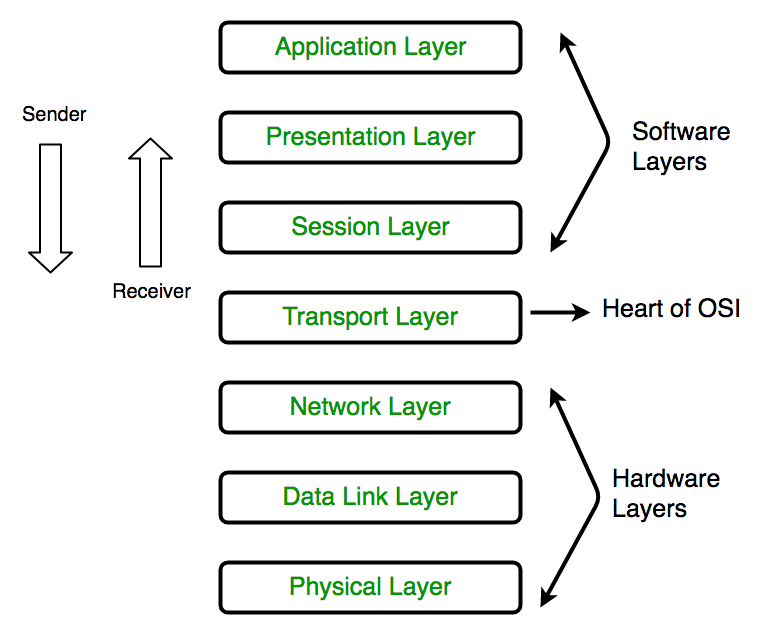
\includegraphics[scale=0.32]{OSI-model-layers}
	\caption{OSI layers, from \cite{GeeksForGeeks:OSI-model}}
\end{figure}


\section{Existing transport implementations}
Previous section mentioned the terms of semantic and temporal transparency. Consequently, there exist two different transport layer implementations, one for each transparency type. \\

The first protocol, which implements semantic transparency, is called TCP (Transmission Control Protocol)\footnote{https://datatracker.ietf.org/doc/html/rfc793}. TCP abstracts away the concept of computer network and exposes a simple interface to the user, where writing bytes is almost the same as writing to a simple binary file. \\

The second protocol, which implements temporal transparency, is called UDP (User Datagram Protocol)\footnote{https://datatracker.ietf.org/doc/html/rfc768}. UDP is a protocol that implements a thin layer of abstraction over the network layer.

\begin{figure}[h!]
	\centering
	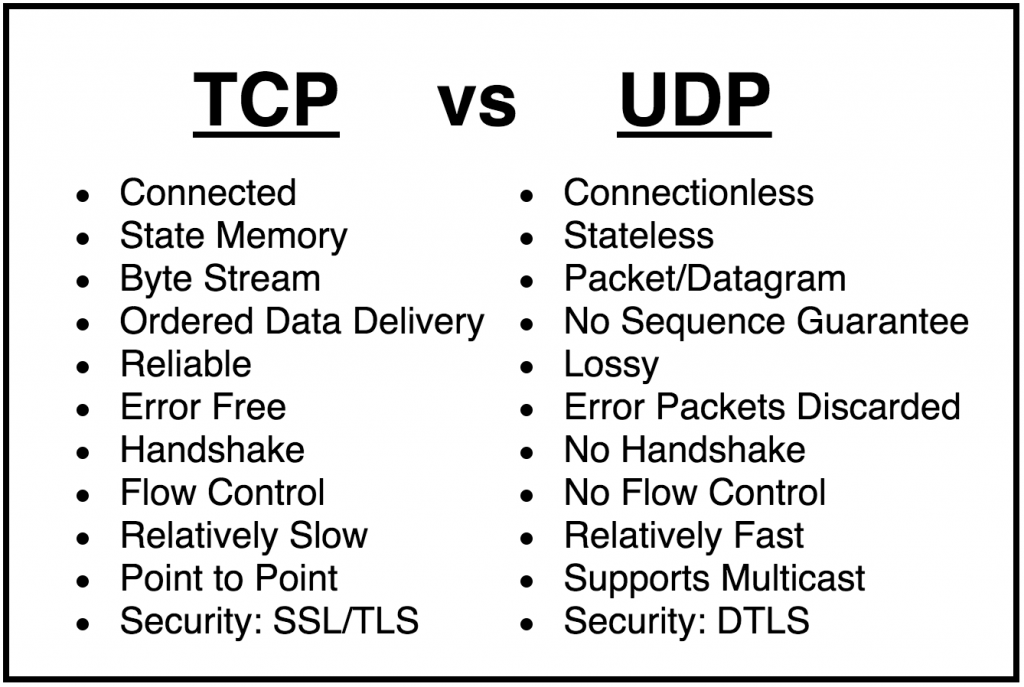
\includegraphics[scale=0.5]{TCP-vs-UDP}
	\caption{Comparison between TCP and UDP protocols, from \cite{NetBurner:TCP-vs-UDP}}
\end{figure}


\section{Custom transport implementation}
While TCP and UDP are great at solving their own use-cases, there exists a major problem: each protocol solves only one type of transparency. With the rise of online gaming, there appeared the need for having both transparency implementations at once; some data would require reliability and ordering that TCP provides (for example, textual chat messages), while other types needed only latest data without the guarantee of delivery (for example, position of the player in a virtual world). \\

Using both protocols at the same time, based on the type of data, is not an ideal solution either, for multiple reasons \cite{GafferOnGames:UDP-vs-TCP}:

\begin{enumerate}
	\item Using TCP can induce packet loss in UDP packets as routers often prioritize TCP segments (as dropping TCP segment requires re-sending, while dropping UDP packet does not).
	\item Supporting many reliable channels (for example, one channel for text message data, another for images or audio) would require many TCP connections, quickly exhausting operating system resources.
	\item Application code-base would be hard to manage, potentially resulting in slower development and harder to track bugs.
\end{enumerate}

For all of those reasons, a custom solution is required - one that allows the user to easily specify, on per packet basis, how data should be delivered. If data is time-sensitive, user must be able to send it in unreliable manner, where temporal transparency is preserved. If data is important and must be delivered, semantic transparency must be preserved. As UDP already provides temporal transparency, we simply need to upgrade it with optional semantic transparency features that are present in the TCP. Implementations of such protocols are often called RUDP - \textit{Reliable User Datagram Protocol}. The rest of this chapter explains one such implementation.

\chapter{Uvod}
Uvod rada. Nakon uvoda dolaze poglavlja u kojima se obrađuje tema.

\chapter{Zaključak}
Zaključak.

\bibliography{literature}
\bibliographystyle{fer}

\begin{sazetak}
Sažetak na hrvatskom jeziku.

\kljucnerijeci{Ključne riječi, odvojene zarezima.}
\end{sazetak}

\engtitle{Development and application of a videogame multiplayer networking library}
\begin{abstract}
Abstract.

\keywords{Keywords.}
\end{abstract}

\end{document}
